\documentclass[twocolumn]{article}
\usepackage[utf8]{inputenc}
\usepackage[margin=1.0in]{geometry}
\usepackage{amsmath, amsfonts}
\usepackage{tikz}
\usepackage[english]{babel}
\usepackage{amsthm}
\usepackage{enumitem}
\usepackage{graphicx}
\usepackage{fancyhdr}
\usepackage{subcaption}
\usepackage{float}

\newcommand{\bd}{\textbf}

\pagestyle{fancy}
\fancyhf{}
\title{Confirming Bragg's Law using X-Ray Diffraction from NaCl}
\author{Kale Stahl}
\lhead{X-Ray Diffraction from NaCl}
\makeatletter
\chead{\@date}
\rhead{\@author}
\makeatother

\begin{document}
	%Makes fancy title
	\makeatletter
	\begin{center}
		{\centering \Large \bd \@title}\\
		\vspace{.5cm}
		{\large \@author}
		\vspace{.25cm}
	\end{center}
	\makeatother
	\begin{abstract}
		This report has the goal of confirming Bragg's law using x-ray diffraction from an NaCl crystal. The experiment was conducted and the results show that Bragg's law holds for such a crystal in general, but further error analysis is needed.
	\end{abstract}
	\section{Introduction}
		The arrangement of atoms or ions in crystals can be understood as an array of parallel lattice. These lattices will form planes in which waves can be scattered, creating a spherical wavelet. In this situation, our wavelength $\lambda$ of the incident wave is unchanged and 
		
		Bragg's law states that the glancing angle $\theta$ is related to an integer multiple of the incident wavelength $\lambda$ in the following way
		\begin{equation}
			n\lambda = 2d\sin \theta \label{bragg's law}
		\end{equation}
		In essence, this means that with a fixed $\lambda$ there exists some $\theta$ that depends on $d$, the distance between objects in the lattice, in which we have that the angle of incidence is equal to the angle of reflection.
		
	\section{Experimental Procedure}
		\subsection{Apparatus}
		We will use the Lehr-und Didaktiksysteme X-ray Apparatus 554 800 (Figure \ref{apparatus}) with serial number 469703. A visualization of this apparatus is seen in Figure \ref{apparatus}. This apparatus is equipped with a built in X-ray tube, goniometer, and Geiger-M\"uller counter, We will detail the exact specifications and use of each of these components below.
		\begin{figure}[h!]
			\begin{center}
				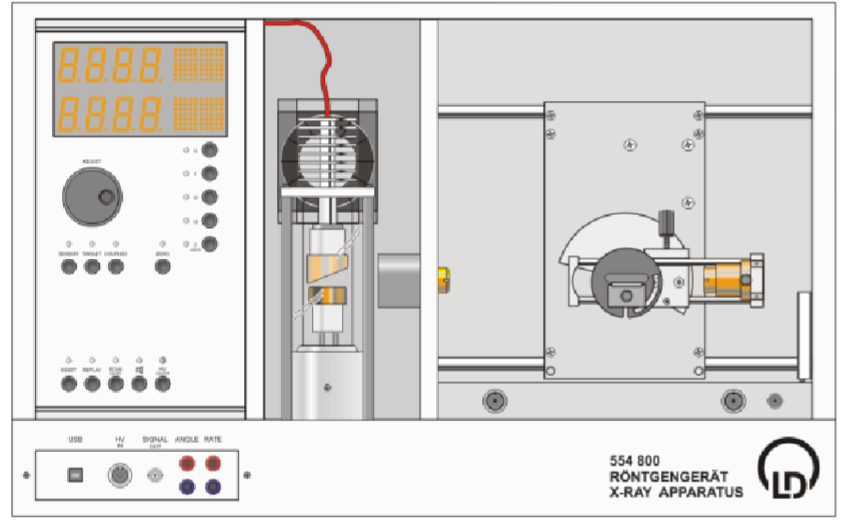
\includegraphics[width = .45\textwidth]{apparatus}
			\end{center}
			\caption{Visualization of the Lehr-und Didaktiksysteme X-ray Apparatus 554 800}
			\label{apparatus}
		\end{figure}
			The X-ray tube(Figure \ref{x-ray tube}) uses a molybdenum anode in a copper block whose purpose is to dissipate heat. This molybdenum has $K_\alpha = 17.4$ keV and $K_\beta = 19.6$ keV.
			\begin{figure}[h!]
				\begin{subfigure}{.45\textwidth}
					\begin{center}
						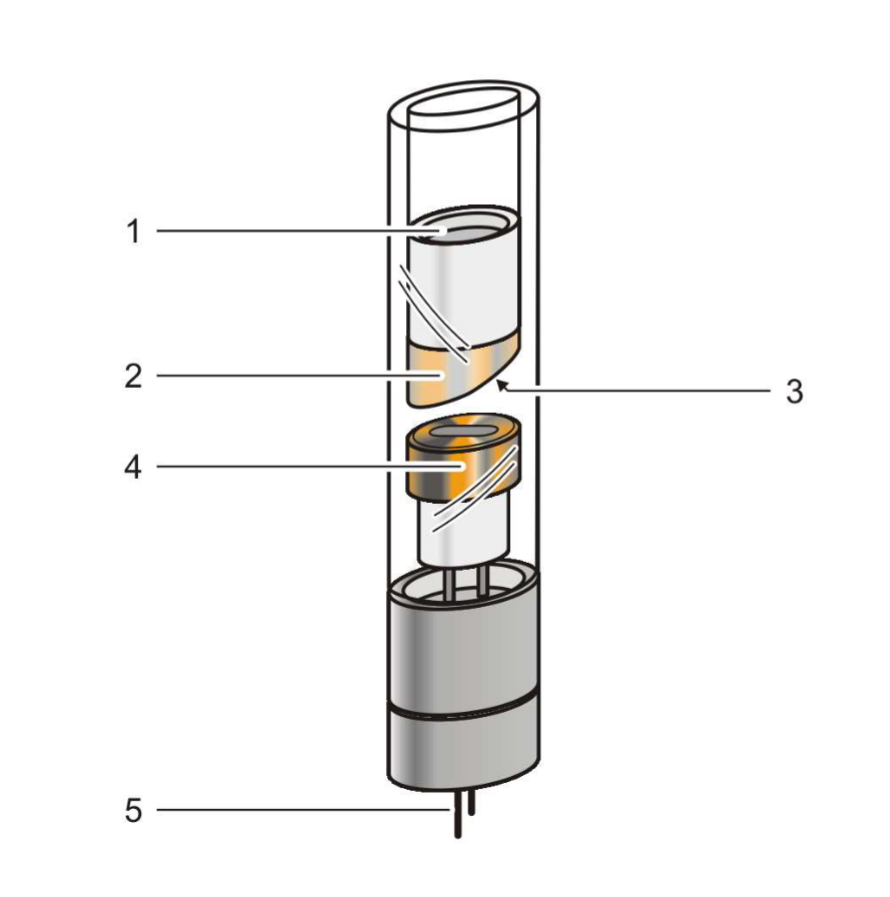
\includegraphics[width = .5\textwidth]{x-ray tube}
					\end{center}
					\caption{Labeled visualization of the x-ray tube. Numbered components are as follows: \bd{(1)} Thread for heat sink; \bd{(2)} Copper block; \bd{(3)} Molybdenum anode; \bd{(4)} Hot cathode; \bd{(5)} Pin socket Base }
					\label{x-ray tube}
				\end{subfigure}
				\hspace{.05\textwidth}
				\begin{subfigure}{.45\textwidth}
					\begin{center}
						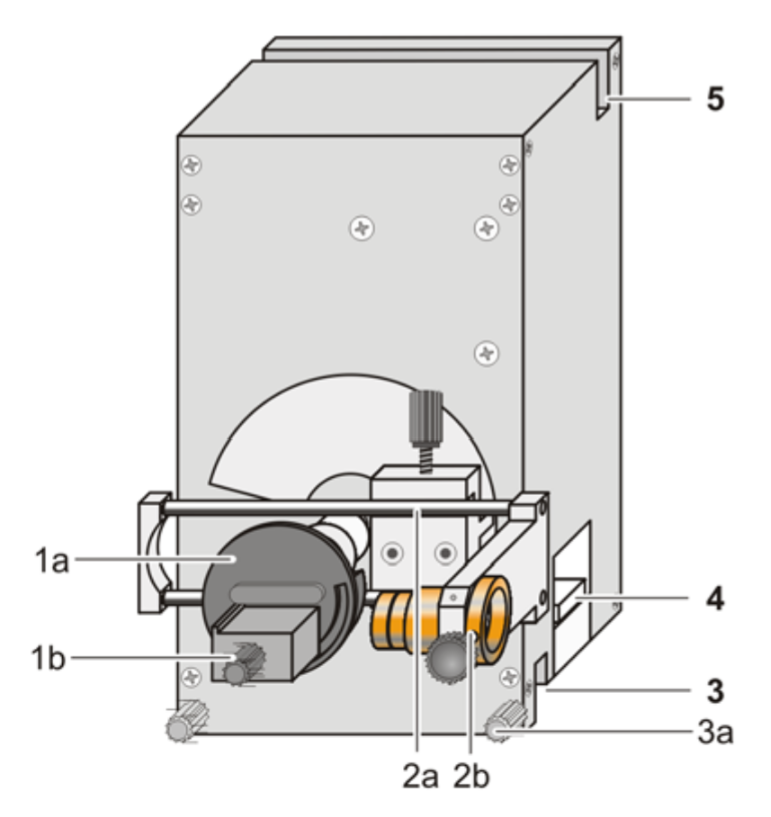
\includegraphics[width = .5\textwidth]{goniometer}
					\end{center}
					\caption{Labeled visualization of the goniometer. Numbered components are as follows: \bd{(1)} Target arm; \bd{(2)} Sensor arm; \bd{(3)} Bottom guide groove; \bd{(4)} Terminal pin connector; \bd{(5)} Top guide groove }
					\label{goniometer}
				\end{subfigure}
				\caption{Descriptions of x-ray tube and goniometer}
			\end{figure}
			This goniometer (Figure \ref{goniometer}) is a self-contained unit for mounting the crystal sample and the detector. It is internally calibrated so that the GM Counter will move twice the angle of the sample for each rotation in order to maintain the Bragg angle. The goniometer has unlimited angle range with an angular resolution of $0.1^\circ$. We will utilize a self-quenching Geiger-M\"uller counter with a thin mica window $d = 12- 15$ mm with a filling of neon, argon, and halogen gas. This will be used to detect the x-ray radiation scattering off the crystal.	The NaCl crystal we will use is a 25 by 25 by 4 millimeter NaCl crystal with the spacing of lattice planes being 282 pm. This crystal has theoretical reflection angles of $7.24^\circ$ for $K_\alpha$ and $6.43^\circ$ for $K_\beta$ from the molybdenum x-ray tube.
		\subsection{Data Collection}
			Data collection will be done using the Geigar-M\"uller counter to measure the number of incident X-rays and the goniometer to measure the angle of the sample. The built in scan mode of the apparatus will be used to scan through the angles of $2^\circ$ and $25^\circ$. The Geigar-Mu\"ller counter will take counts of how many X-ray photons per second it detects at that angle. The data can be collected directly from the device utilizing its built in software. We will then plot the count rate as a function of angle in which we should see defined peaks at each Bragg for each value of $n$ for Mb $K_\alpha$ and $K_\beta$ emissions. We expect there to be six defined peaks, one for the $3$ values of $n$ for each emission spectrum. We will then fit a curve to these emission peaks in order to find the angle in which they are maximized, which will be our Bragg angle for that emission line.
	\section{Data Analysis}
			The first step in taking data is to see the expected counters of the GM counter without a sample to diffract off of. The purpose of this is to determine the shape of the expected peak that will be superimposed on the X-ray emission spectrum of molybdenum. This experiment was carried out with a sample timer of 10 seconds.
			\begin{figure}
				\centering
				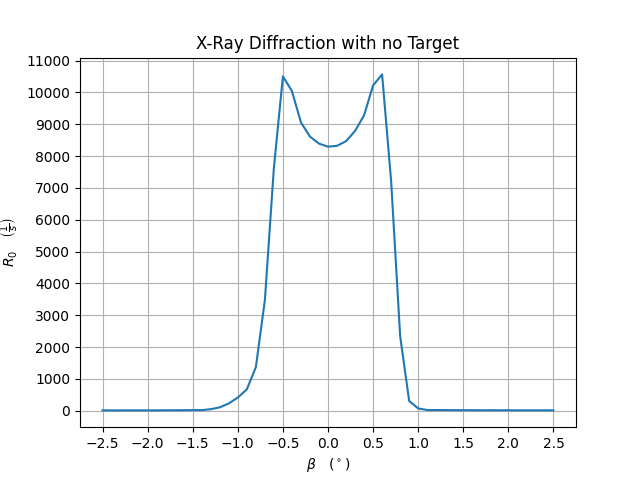
\includegraphics[width = .5\textwidth]{../Graphs/ZeroData}
				\caption{X-ray count data without a sample}
				\label{zerodata}
			\end{figure}
			Our results for this baseline can be seen in Figure \ref{zerodata}. The dip in the peak of the curve is most likely due to the fact that there is a lip on the sample rest and this caused the x-rays to scatter abnormally. Otherwise, we have a curve that fits very similarly to a Gaussian, so we will utilize a Gaussian fit for each peak in our experimental data. 
			
			With our fit determined, we will now analyze the data of the full scan. The graph of the full gamut of data is seen in Figure \ref{fulldata}. In this scan, with a sample timer of 10 seconds, we can clearly see 6 defined peaks. These peaks represent the angles in which the count of x-rays is maximized, meaning this is the point of the total constructive interference which is interpreted as the Bragg angle. Thus, to determine our Bragg angle for each peak, we will collect data on each peak individually and then fit a modified Gaussian to each peak and interpret the center of the Gaussian to be our maximal angle.
			
			To fit our data, we first collected data using a sample timer of 20 seconds to improve our precision of each peak. Then, we determined which points we could consider part of the peak and which can be considered part of the background data. Once this is determined, we can then fit a function to only the background data, and the shift our peak fit by the fit of the background in order to ensure that our fit accurate. For this case, we fit a cubic polynomial $P_3(x)$ to the background data and then from there used the fit seen in (\ref{eq: fit}) to find our function $f(x)$ with parameters $a, b, c$ with $b$ giving us the point of maximality for our specific peak.
			\begin{equation}
				f(x) = ae^{\frac{-(x-b)^2}{c^2}} + P_3(x) \label{eq: fit}
			\end{equation}	
			Our fitted data for the $K_\beta$ emission lines can be seen in Figure \ref{fig: beta} and the fitted data for $K_\alpha$ is given by the peaks seen in Figure \ref{fig: alpha}.
			\begin{figure}
				\centering
				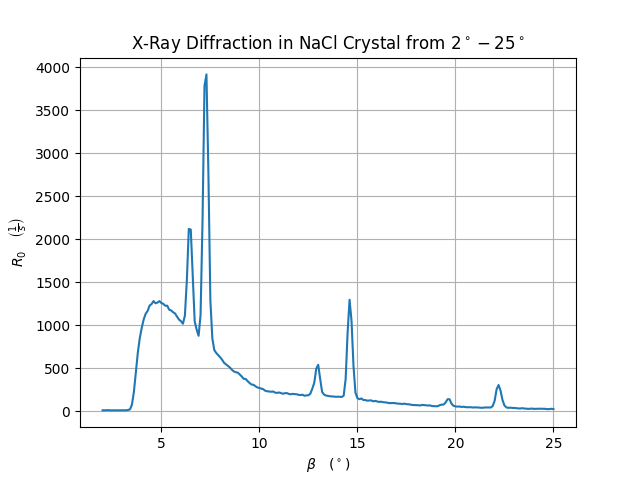
\includegraphics[width = .5\textwidth]{../Graphs/FullData}
				\caption{Graph of count rate versus angle }
				\label{fulldata}
			\end{figure}
			
			\begin{figure}[h!]
				\begin{subfigure}{.33\textwidth}
					\begin{center}
						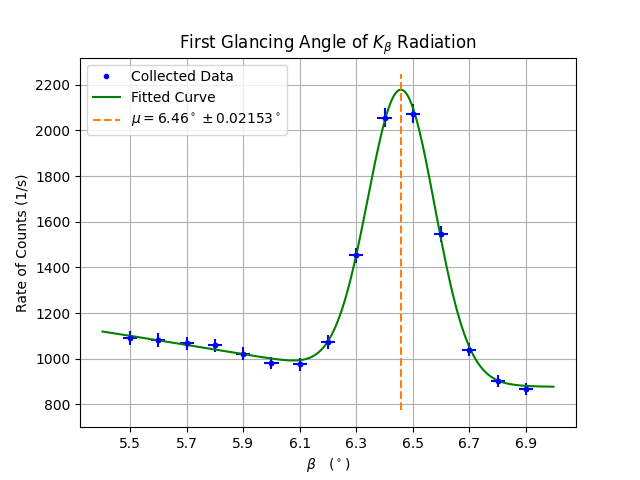
\includegraphics[width = \textwidth]{../Graphs/Peak 1}
					\end{center}
					\label{beta 1}
				\end{subfigure}
				\begin{subfigure}{.33\textwidth}
					\begin{center}
						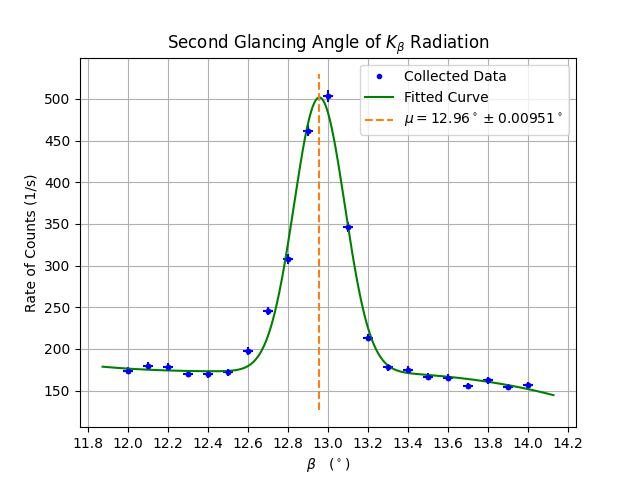
\includegraphics[width = \textwidth]{../Graphs/Peak 3}
					\end{center}
					\label{beta 2}
				\end{subfigure}
				\begin{subfigure}{.33\textwidth}
					\begin{center}
						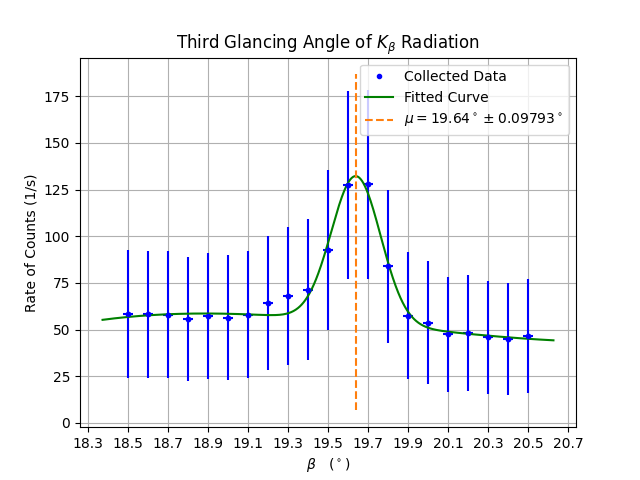
\includegraphics[width = \textwidth]{../Graphs/Peak 5}
					\end{center}
					\label{beta 3}
				\end{subfigure}
				\caption{Graphs of each peak of the Mb $K_\beta$ emission.}
				\label{fig: beta}
			\end{figure}
			
			\begin{figure}[h!]
				\begin{subfigure}{.33\textwidth}
					\begin{center}
						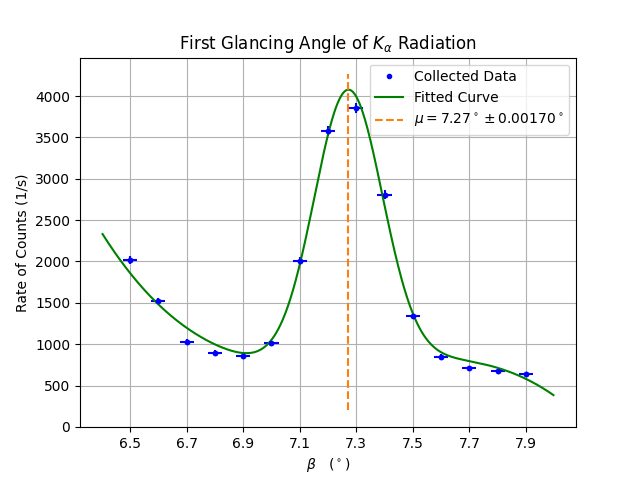
\includegraphics[width = \textwidth]{../Graphs/Peak 2}
					\end{center}
					\label{alpha 1}
				\end{subfigure}
				\begin{subfigure}{.33\textwidth}
					\begin{center}
						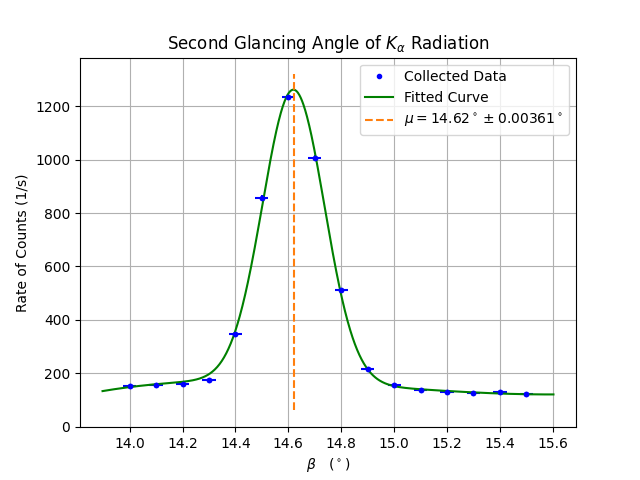
\includegraphics[width = \textwidth]{../Graphs/Peak 4}
					\end{center}
					\label{alpha 2}
				\end{subfigure}
				\begin{subfigure}{.33\textwidth}
					\begin{center}
						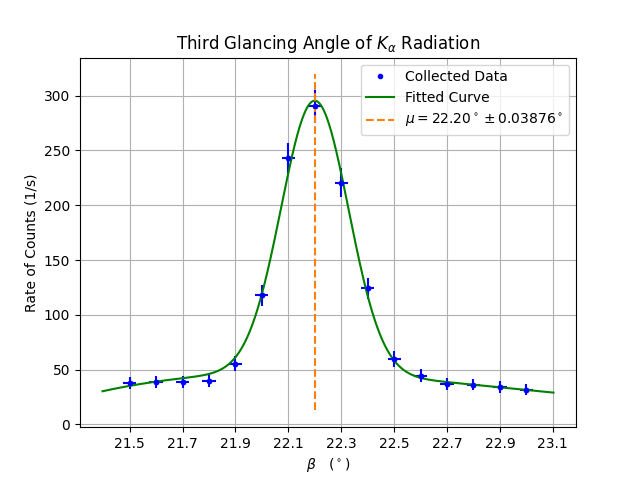
\includegraphics[width = \textwidth]{../Graphs/Peak 6}
					\end{center}
					\label{alpha 3}
				\end{subfigure}
				\caption{Graphs of each peak of the Mb $K_\alpha$ emission.}
				\label{fig: alpha}
			\end{figure}
		\begin{figure}
			\centering
			\begin{tabular}{|c|c|c|}
				\hline
				$\mathbf{n}$ & $\boldsymbol{\theta}(\mathbf{K}_{\boldsymbol{\beta}})$ & $\boldsymbol{\theta}(\mathbf{K}_{\boldsymbol{\alpha}})$\\
				\hline
				1& $6.42^\circ$& $7.24^\circ$\\
				2& $12.93^\circ$& $14.60^\circ$\\
				3& $19.61^\circ$& $22.21^\circ$\\
				\hline
			\end{tabular}
			\caption{Accepted values for glancing angles}
			\label{truevalue}
		\end{figure}
		\begin{figure}
			\centering
			\begin{tabular}{|c|c|c|}
				\hline
				$\mathbf{n}$ & $\boldsymbol{\theta}(\mathbf{K}_{\boldsymbol{\beta}})$ & $\boldsymbol{\theta}(\mathbf{K}_{\boldsymbol{\alpha}})$\\
				\hline
				1& $6.46^\circ\pm 0.00379^\circ$&$7.27^\circ\pm 0.00420^\circ$\\
				2& $12.96^\circ\pm 0.00951^\circ$&$14.62^\circ\pm 0.00361^\circ$\\
				3& $19.64^\circ\pm 0.0162^\circ$&$22.20^\circ\pm 0.00707^\circ$\\
				\hline
			\end{tabular}
			\caption{Measured values for glancing angles}
			\label{foundvalue}
		\end{figure}
			
	\section{Results and Conclusions}
	\newpage
	\section*{References}
	
\end{document}